\documentclass[border=8pt]{standalone}
\usepackage[T1]{fontenc}\usepackage[utf8]{inputenc}
\usepackage{helvet}\renewcommand{\familydefault}{\sfdefault}
\usepackage{tikz,xcolor}
\usetikzlibrary{arrows.meta,positioning,shapes.geometric,shapes.multipart,calc,fit,backgrounds,decorations.markings}
\definecolor{ink}{HTML}{1E1B16}\definecolor{paper}{HTML}{FBF8F2}\definecolor{clay}{HTML}{B5482A}\definecolor{soft}{HTML}{F1E9DA}\definecolor{pine}{HTML}{24402F}
\tikzset{
  every node/.style={font=\small,text=ink},
  >=Stealth, line/.style={draw=ink,line width=0.8pt},
  cls/.style={rectangle split,rectangle split parts=3,draw=ink,line width=0.8pt,fill=soft,align=left,inner xsep=6pt,inner ysep=4pt,
              rectangle split part align={center,left,left},minimum width=3.0cm},
  cls2/.style={rectangle split,rectangle split parts=2,draw=ink,line width=0.8pt,fill=soft,align=left,inner xsep=6pt,inner ysep=4pt,
              rectangle split part align={center,left},minimum width=3.0cm},
  box/.style={rectangle,draw=ink,line width=0.8pt,fill=soft,align=center,inner sep=5pt,minimum height=0.8cm},
  state/.style={rectangle,rounded corners=8pt,draw=ink,line width=0.8pt,fill=soft,align=center,inner sep=6pt,minimum width=2.2cm,minimum height=0.9cm},
  act/.style={rectangle,rounded corners=10pt,draw=ink,line width=0.8pt,fill=soft,align=center,inner sep=5pt,minimum width=2.4cm,minimum height=0.8cm},
  dec/.style={diamond,draw=ink,line width=0.8pt,fill=soft,inner sep=1pt,minimum width=0.9cm,minimum height=0.9cm},
  uc/.style={ellipse,draw=ink,line width=0.8pt,fill=soft,align=center,inner sep=3pt,minimum width=3.2cm,minimum height=1.0cm},
  note/.style={rectangle,draw=ink,line width=0.6pt,fill=yellow!12,align=left,inner sep=4pt,font=\footnotesize},
  lab/.style={font=\footnotesize,fill=paper,inner sep=1.5pt},
  err/.style={},
}
\newcommand{\actor}[3]{% x,y,label
  \draw[line width=0.8pt] (#1,#2+0.55) circle (0.17);
  \draw[line width=0.8pt] (#1,#2+0.38)--(#1,#2-0.15) (#1-0.3,#2+0.22)--(#1+0.3,#2+0.22) (#1,#2-0.15)--(#1-0.25,#2-0.6) (#1,#2-0.15)--(#1+0.25,#2-0.6);
  \node[font=\small] at (#1,#2-0.9) {#3};}
\begin{document}
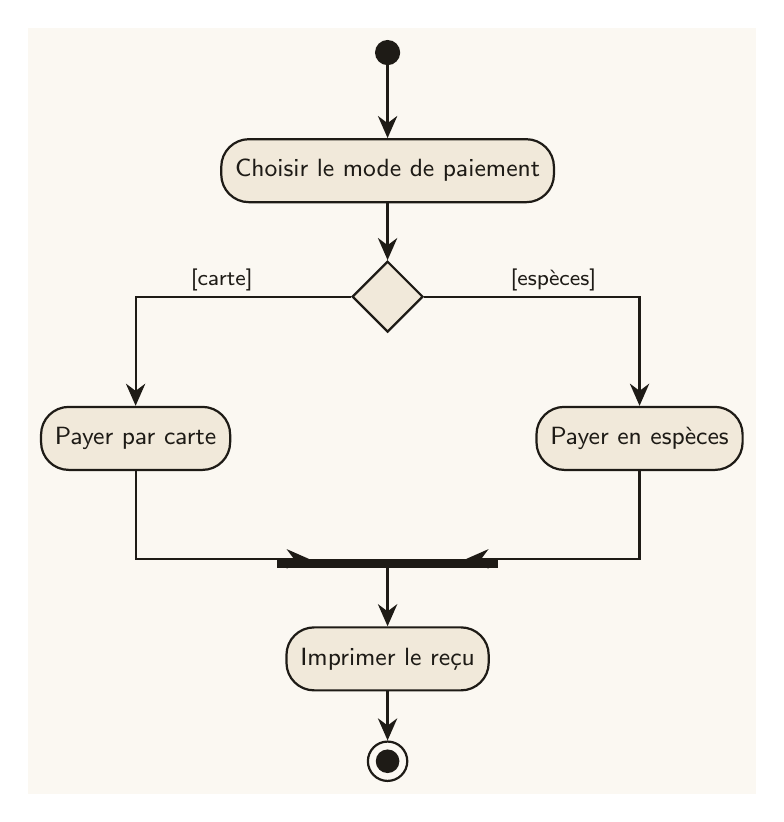
\begin{tikzpicture}[background rectangle/.style={fill=paper},show background rectangle]
\fill[ink] (0,0) circle (0.16);
\node[act,minimum width=4.2cm] (m) at (0,-1.5) {Choisir le mode de paiement};
\node[dec] (d) at (0,-3.1) {};
\node[act] (c) at (-3.2,-4.9) {Payer par carte};
\node[act] (e) at (3.2,-4.9) {Payer en esp\`eces};
\fill[ink] (-1.4,-6.55) rectangle (1.4,-6.43);
\node[act] (r) at (0,-7.7) {Imprimer le re\c{c}u};
\node[circle,draw=ink,line width=0.8pt,minimum size=0.5cm] (fi) at (0,-9.0) {};\fill[ink] (fi) circle (0.15);
\draw[line,-{Stealth[length=8pt,width=7pt]}] (0,-0.16)--(m.north);
\draw[line,-{Stealth[length=8pt,width=7pt]}] (m.south)--(d.north);
\draw[line,-{Stealth[length=8pt,width=7pt]}] (d.west)-|(c.north) node[pos=0.3,above,lab]{[carte]};
\draw[line,-{Stealth[length=8pt,width=7pt]}] (d.east)-|(e.north) node[pos=0.3,above,lab]{[esp\`eces]};
\draw[line,-{Stealth[length=8pt,width=7pt]}] (c.south)|-(-1.0,-6.43);
\draw[line,-{Stealth[length=8pt,width=7pt]}] (e.south)|-(1.0,-6.43);
\draw[line,-{Stealth[length=8pt,width=7pt]}] (0,-6.55)--(r.north);
\draw[line,-{Stealth[length=8pt,width=7pt]}] (r.south)--(fi.north);
\end{tikzpicture}
\end{document}
